\begin{figure}
    \centering
    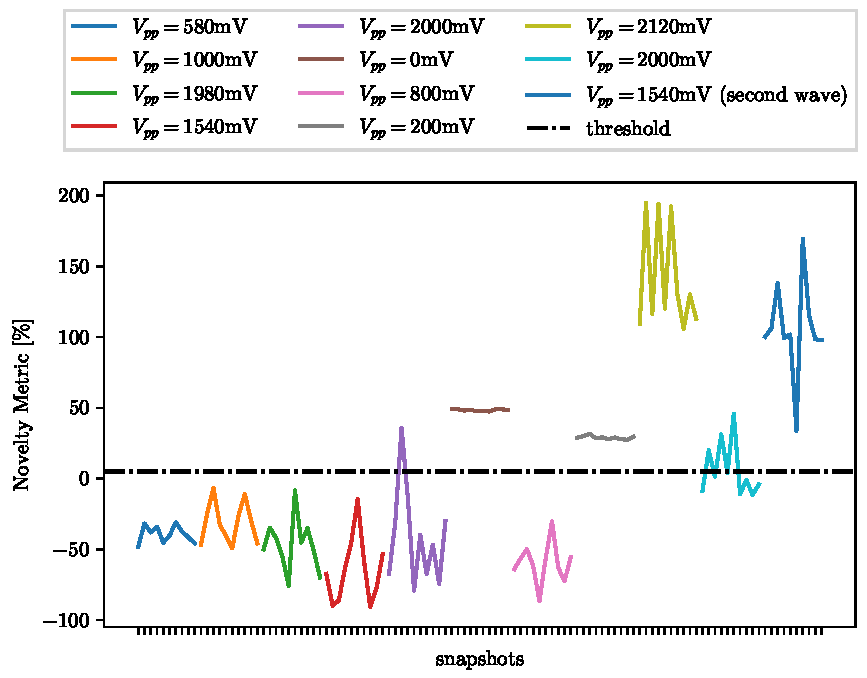
\includegraphics{Images/shaker/Test02.pdf}
    \caption{Novelty detection result}
    \label{fig:shaker_results02}
\end{figure}

\begin{figure}
    \centering
    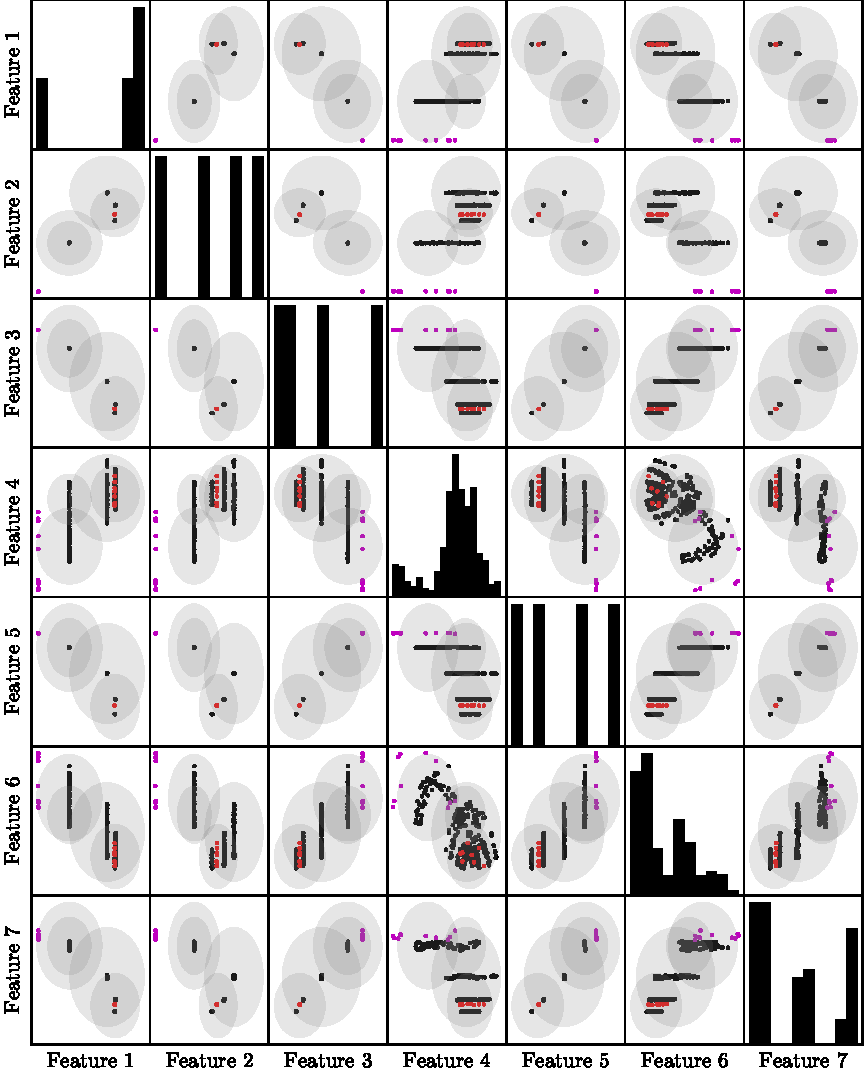
\includegraphics{Images/shaker/ConfusionMatrix.pdf}
    \caption{False Negative and True Positive results. On the diagonal there is an hystogram of the feature values. The off-diagonal plots are the scatter plots of the features. The shades are the projection of the clusters on the considered plane. (Red: False Negative, Magenta: True Positive, Black: training data)}
    \label{fig:shaker_conf_matrix}
    \end{figure}